% ============================================================================
%  BLOQUE I — DIAPOSITIVAS 2–3: ÍNDICE + INTRODUCCIÓN
% ============================================================================

% ----------------------------------------------------------------------------
%  DIAPOSITIVA 2 — ÍNDICE
% ----------------------------------------------------------------------------
{
\setbeamertemplate{footline}{}
\begin{frame}{Índice}
  \hypertarget{indice}{}%
  \tableofcontents
\end{frame}
}

\section{Introducción}

% ----------------------------------------------------------------------------
%  DIAPOSITIVA 3 — RESUMEN EJECUTIVO + MOTIVACIÓN
% ----------------------------------------------------------------------------
\begin{frame}{Resumen Ejecutivo y Motivación}
  \begin{columns}[T]
    \column{0.48\textwidth}
    \IfFileExists{figures/03_arquitectura.pdf}{%
      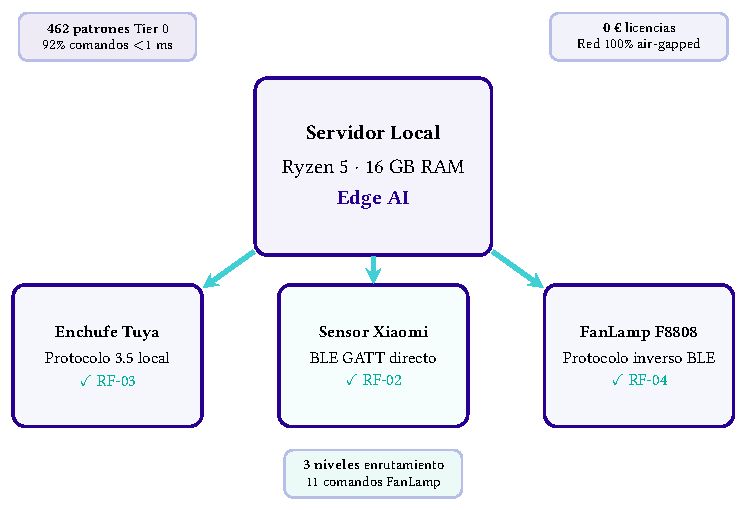
\includegraphics[width=\textwidth, height=3.8cm, keepaspectratio]{figures/03_arquitectura.pdf}%
    }{
      \textcolor{darkgray}{[Figura: panorama del sistema]}
    }

    \vspace{0.15cm}
    \begin{block}{¿Qué es Luxe Core AI?}
      \footnotesize
      Sistema 100\% local de control de confort térmico orquestado por IA en el \textit{edge}.
      \textbf{462 patrones} Tier~0 (92\%, $<$1 ms) · \textbf{0 €} licencias · Red air-gapped.
    \end{block}

    \column{0.52\textwidth}
    \IfFileExists{figures/04_motivacion.pdf}{%
      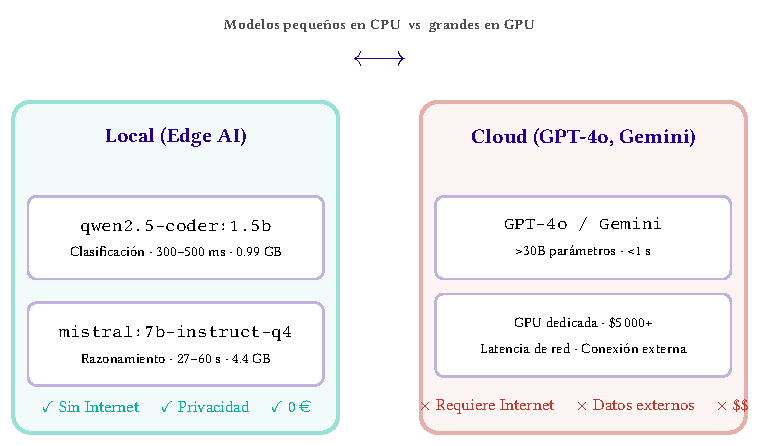
\includegraphics[width=\textwidth, height=3.8cm, keepaspectratio]{figures/04_motivacion.pdf}%
    }{
      \textcolor{darkgray}{[Figura: comparativa Local vs Cloud]}
    }

    \vspace{0.15cm}
    \begin{exampleblock}{Principio rector}
      \footnotesize
      La tecnología del hogar no debería exigir ceder la privacidad a cambio de comodidad.
    \end{exampleblock}
  \end{columns}
\end{frame}
